\documentclass[english]{article}
%\usepackage[round]{natbib}
\usepackage{amsfonts}
\usepackage{amsmath}
\usepackage{paralist}
\usepackage{subfig}
\usepackage{times}
\usepackage{latexsym}
\usepackage{graphicx}
\usepackage[T1]{fontenc}
\usepackage{tikz}
\usepackage{url}
\usepackage{pgfplotstable}
\usepackage{titlesec}
\usepackage{color}
\usepackage{lipsum,adjustbox}
\usepackage[font={small}]{caption}
\usetikzlibrary{positioning}

\usepackage{acl2017}
\graphicspath{{./plots/}}
\newcommand{\oa}[1]{\footnote{\color{red}OA: #1}}
\newcommand{\lc}[1]{\footnote{\color{green}LC: #1}}
\begin{document}
	
\title{The Intricacies of Reference-based Evaluation in Grammatical Error Correction}

\author{
  Leshem Choshen\textsuperscript{1} and Omri Abend\textsuperscript{2} \\
  \textsuperscript{1}School of Computer Science and Engineering,
  \textsuperscript{2} Department of Cognitive Sciences \\
  The Hebrew University of Jerusalem \\
  \texttt{leshem.choshen@mail.huji.ac.il, oabend@cs.huji.ac.il}\\
}


\maketitle

\begin{abstract}
	
\end{abstract}

\section{Introduction}

% Error correction 
% evaluation in error correction and its centrality
% faithfulness to the source meaning is important, and this has been noted but prev work, and evaluation is geared towards it
% gap in evaluation: however, steps taken to ensure conservativeness in fact push towards formal conservativism by their definition (theoretical claim about the measure)
% this may result in systems that make few changes. indeed we find that this is the case (empirical claim about systems)

% we pursue two approaches to overcome this bias.

% 1. increasing the number of references. this has been proposed before and pursued with m=2, but no assessment of its sufficiency or its added value over m=1 has been made. In order to address this gap we first charachterize the distribution of possible corrections for a sentence. We leverage this characterization to characterize the distribution of the scores as a function of $m$, and consequently assess the biases introduced by taking $m=1,2$ as with previous approaches. 
% We find that taking these values of $m$ drammatically under-estimate the system scores. 
% We back our analysis of these biases with an analysis of the variance of these estimators.
% We analyze the two commonly used scores, the M2 score often used for evalauted, and the accuracy score commonly used in training.

% 2. we note that in fact the important factor is semantic conservativism and explore means to directly assess how semantically conservative systems here through the use of semantic annotation. 
% We use the UCCA scheme as a test case, motivated by HUME.
% First question: is it well-defined on learner language. it is.
% Second question: are corrections in fact semantically conservate? to show that, we need to verify that the corrections make few (if any) semantic changes. our results indicate that this is the case: we show that the corrections are similar in (UCCA) structure to the source.

% conclusion (not in intro): we tried to use semantic similarity to improve systems. this is difficult due to semantic conservatism. we expect this will be in issue once evaluation is improved. future work.
% also future work: use multiple references in training (did people do that?)

% sections:
% 1. Introduction
% 2. Formal conservativism in GEC
% 3. First approach: Multiple References
% 3.1. A Distribution of Corrections
% 3.2. Scores (M2, accuracy index, accuracy exact)
% 3.3. Data
% 3.4. Bias of the Scores (setup + results)
% 3.5. Variance of the Scores (setup + results)
% 4. Second approach: Semantic Similarity
% 4.1. Semantic Annotation of Learner Language (prev work)
% 4.2. UCCA Scheme (see HUME)
% 4.3. Similarity Measures (including prev work of elior)
% 4.4. Empirical Validation: IAA, semantic conservativism vs. gold std
% 5. Conclusion

Grammatical Error Correction (GEC) is a challenging research field, which interfaces with many
other application areas of linguistics. This interest is reflected in the four recent shared
tasks that were devoted to GEC: HOO-2011 and 2012 \cite{dale2011helping,dale2012hoo},
the CoNLL 2013 and 2014 shared tasks \cite{kao2013conll,ng2014conll}.
Within GEC, considerable effort has been placed on the difficult task of
evaluation \cite{tetreault2008native,madnani2011they,chodorow2012problems,dahlmeier2012better}.
Much like in machine translation, evaluation in GEC poses considerable difficulties, much
due to the multiple valid corrections each source sentence may have.

An important criterion in the evaluation of GEC systems (henceforth, {\it correctors})
is their ability to
generate corrections that are faithful to meaning of the source. In fact, many would prefer
a somewhat cumbersome or even an occasionally ungrammatical correction over a correction
that alters that meaning of the source \citet{brockett2006correcting}.
Indeed, when manually compiling the gold-standard corrections for the HOO corpus, annotators
were instructed to be conservative in their corrections\footnote{Daniel Dahlmeier,
  personal communication.}.
A recent attempt to formally capture this precision/recall asymmetry has been the shift from
using $F_1$ to $F_{0.5}$, where Precision is emphasized over Recall, as a common evaluation
measure in GEC \cite{dahlmeier2012better}.

However, favoring precision over recall may lead to reluctance of GEC systems to make any
changes. Using a single reference correction (as is the common practice in GEC) compounds
this problem, as systems are not only penalized more for making an incorrect change (over not making
any change), but are also penalized for any correct change not found in the reference.
We present results that indicate that this is the case. Evaluating the output of 15 state of the art
GEC systems that participated in the recent CoNLL2014 shared task, we see that all of them
grossly underestimate the number of corrections that need to be made, relative to the human references
(\S\ref{sec:formal_conservatism}). 

We pursue two approaches to address this gap, by developing improved reference-based
similarity measures (or simply {\it measures} for brevity) for assessing 
the quality of a correction, which are less biased towards conservatism:
(1) increasing the amount of references (henceforth, $M$) (\S\ref{sec:increase-reference}),
and (2) and developing a semantic similarity measure, which measures the semantic relatedness
between the system's output and the reference, rather than their similarity
as strings (\S\ref{sec:Semantics}). Such improved measures can be used as
loss functions in the training regime or as evaluation measures,
thus addressing the observed conservatism.

Increasing the number of references was previously pursued with $M=2$,
but no empirical assessment of its sufficiency or its added value over $M=1$ has been made.
In order to address this gap we first estimate the number of corrections necessary in order
to cover the bulk of the distribution of possible corrections.
We then consider two prominent measures for assessing the validity of a proposed correction
relative to a set of references: the GEC $F$ score often used for evaluation \cite{dahlmeier2012better},
and the 0-1 measure (accuracy) commonly used as a loss function in training GEC systems.
Specifically, we characterize the distribution of the measures' scores
as a function of $M$, and consequently assess the biases introduced by taking $M=1$ or $M=2$
as with previous approaches. 
We find that assessment based on these values of $M$ dramatically under-estimate the
true performance of the systems (\S\ref{sec:increase-reference}). 
The analysis of this bias is backed with an analysis of the variance of these estimators.

We further pursue an alternative way of determining whether a correction faithfully
represents the semantics of the source, by developing a semantic measure based on the similarity
in their semantic structures. We define a measure using the UCCA scheme \cite{abend2013universal} as a
test case, motivated by the recent use of the scheme for machine translation evaluation \cite{birch2016hume}.
In order to assess the feasibility of this approach, we annotate a section of the NUS \cite{dahlmeier2013building}
parallel corpus. Our results support the feasibility of the proposed approach,
by showing that semantic structural annotation can be consistently applied
to learner language, as attested by the inter-annotator agreement,
and that the proposed measure assigns a high similarity score between the source and the reference
correction.

We note that the two approaches we pursue are complementary means for addressing the difficulties
incurred by the multitude of ways to correct a sentence, and the consequent inadequacy of assessing
the validity of a proposed correction using its string similarity to a single reference.
The first approach addresses this by attempting to cover the bulk of the distribution of possible
corrections for a sentence, while the second uses semantic instead of string similarity that abstracts
away from some of the formal variation between different corrections.

\section{Conservativism in GEC Systems}\label{sec:formal_conservatism}

%The field of GEC was always thriving for conservatism in its corrections, with the prominent example of using
%$F_{0.5}$ emphasizing precision over recall(\cite{ng2014conll}). we wish to highlight the problem that
%arises from pursuing this conservatism as done today.
%Then, we wished to be conservative, and we achieved that, why shouldn't we rejoice just yet? Theoretically, we might be progressing towards not correcting at all, instead of progressing towards correcting more accurately. 

%Manual analysis showed excessive formal conservatism and under correction.
%Albeit important, manual analysis is not enough and we aimed for generating some quantitative measures. 

We begin by showing evidence that the bias of current measures towards conservatism
has resulted in systems that tend to make too few changes in the source. 

\paragraph{Experimental Setup \label{par:experimental_setup}}

We evaluate conservatism on the NUS dataset \cite{dahlmeier2013building}, a parallel
corpus of learner language(LL) paragraphs and their corrected versions which
has become the de facto standard since its use in the CoNLL 2013 and 2014
shared tasks \cite{kao2013conll,ng2014conll}.
The NUS corpus consists of paragraphs on various topics written by language learners,
each containing about 400 words.

In order to have better evaluation of the real goal of corrections we also
compute all of the measures on the TreeBank of Learner Language \cite{berzak2016universal},
based on the Cambridge First Certificate in English (FCE) \cite{yannakoudakis2011new},
a new large parallel corpus containing only ungrammatical sentences of learners
native of different languages.

We discarded all non alpha-numerics whether within a token or a token on its own.

We conduct our evaluation on all participating systems in the CoNLL 2014,
in addition to the best performing system on this dataset \cite{rozovskaya2014building}.
The particiapting systems and their abbreviations are: Adam Mickiewicz University(AMU), University of Cambridge(CAMB), Columbia University and the University of Illinois at Urbana-Champaign(CUUI), Indian Institute of Technology, Bombay(IITB), Instituto Politecnico NacionalIPN, National Tsing Hua University(NTHU), Peking University(PKU), Pohang University of Science and Technology(POST), Research Institute for Artificial Intelligence, Romanian Academy(RAC), Shanghai Jiao Tong University(SJTU), University of Franche-Comte(UFC)University of Macau(UMC), Rozovskaya and Roth's best performing system (RoRo) \cite{rozovskaya2016grammatical}.

\paragraph{Measures of Conservatism.} There are several ways in which the source and the reference
may diverge. First, individual words may be altered, deleted or added.
Second, the order of the words may be different,
and third, source sentences may be split or concatenated in the reference.
We quantify these divergences using three corresponding measures.

In order to measure sentence splitting/concatenation, we aligned sentences and counted how
many sentences were split and how many concatenated. To align we matched sequentially last
words in sentences.

In order to measure word changes, we first compute word alignment,
and then we count the number of different aligned words,
in addition to the deleted or added words.
For alignment, we note that, unlike in translation,
aligning words is a simple task as most of the words are kept unchanged,
deleted fully, added, or changed slightly. This allows us to
produce word alignment by computing the edit distnace between the tokens.
We formulate the alignment problem as a weighted bipartite graph matching problem,
where each side of the graph corresponds to the tokens of another part of the text.
Given $x_1\ldots x_n,y_1,\ldots y_m$ e weight of each edge is the edit distance between the tokens.\footnote{When breaking ties, we favor alignments where ...}
%To break ties, we add a penalty term. The penalty is always smaller than the minimum cost of one action, favoring a sentence order when a word occurs twice.
This alignment is needed because we only know the final corrections,
a main obstacle that was considered in the assessment methods as well
\cite{dahlmeier2012better}.

Word order differences between the source and corrected sentences is
computed by first aligning tokens as above, and computing Spearman's $\rho$ on the resulting alignment.
$\rho$ is low where the order of tokens is similar on both sides (according to the alignment).


\begin{figure}
	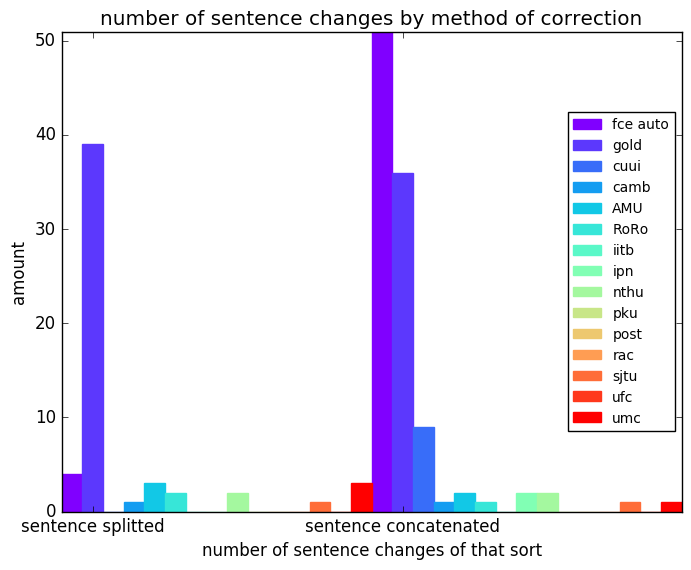
\includegraphics[width = 8cm]{aligned}
	\caption{Number of source sentences (y-axis) splitted (right bars) or concatenated (left bars) in the correction,
          according to
          the gold standard (striped column) and different correctors (colored columns). See \S\ref{par:experimental_setup} for a legend
          of the systems. The gold standard makes about an order of magnitude more splits and
          concatenations than the correctors.}
	\label{fig:split}
\end{figure}

\begin{figure}
	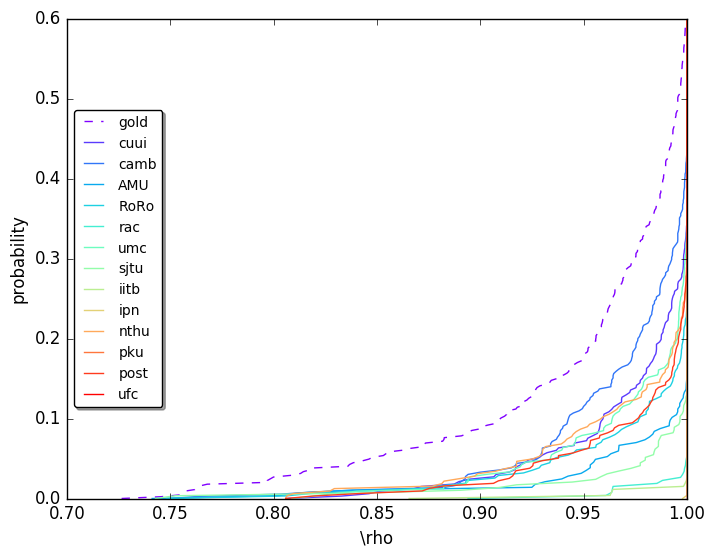
\includegraphics[width = 8cm]{spearman_ecdf}
		\caption{Probability(y-axis) of a sentence to get Spearman's rho values(x-axis) of index alignment by different correctors. See \S\ref{par:experimental_setup} for a legend
		of the systems.
          The gold standard(dotted line) makes word change alterations to more sentences than the correctors,
          and within these sentences, it changes order more substantially.}
	\label{fig:rho}
\end{figure}

\begin{figure}
	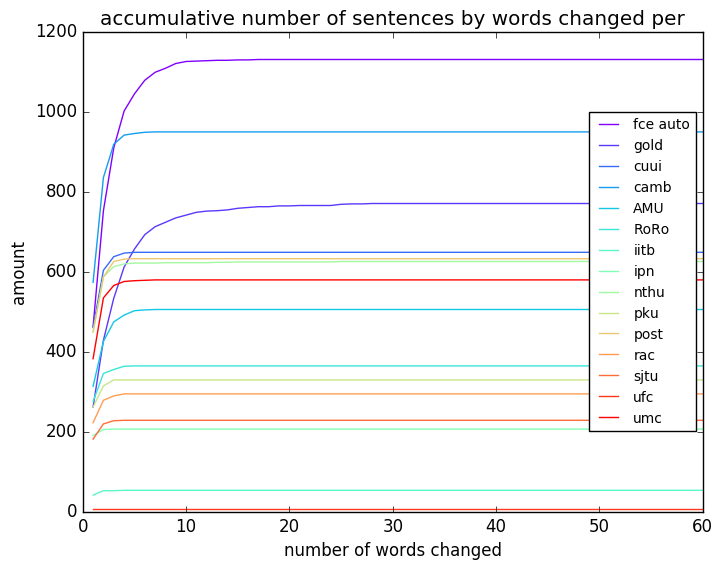
\includegraphics[width = 8cm]{words_differences}
	\label{fig:words_changed}
        \caption{Amount of sentences(heat) by number of words 
        	changed(x-axis) per system(y-label). See \S\ref{par:experimental_setup} for a legend
        	of the systems. The gold standard(bottom) corrects more words per sentences and more sentences relative to other systems.}
\end{figure}

\paragraph{Results.}
Figures \ref{fig:split}, \ref{fig:words_changed}, \ref{fig:rho} present our results using the split and concatenate, number of words changed per sentence and Spearman's row measures respectively.\oa{add here explanation on each of the graphs; don't worry about repeating what you said in the caption}
Results show that the gold standard makes changes to considerably more source sentences than any of the systems, and within the changed sentences, changes more words and makes more word order changes, often an order of magnitude more. For example, in the gold standard there are 44 sentences which have 5 words corrected, the most sentences with only 4 corrections another corrector has is 34.

%starting at what we see isn't changed in the gold standard. We can think of it as what calls for formal conservatism.
%We see that it is most common for a sentence to have no change, not to concatenate two consecutive sentences and not to split a sentence into two. We also observe high correlation coefficient for most of the sentences. Summing it all together we indeed have more unchanged than changed in every measure we have. But, with a closer look we should also notice that it mostly tells us about the dataset. Specifically the level of English found in the dataset.
%These measures should be seen as a gold standard of the amount of corrections to be done, and as we might wish to be a bit conservative and not exceed it, this is still where we should aim.

%When we broaden our view and consider the results of the different correctors, the picture is clear. All correctors are over conservative.
%It is not only that correctors don't tend to overcorrect, they all,to the last one, by all the measures we checked, undercorrect a lot
%and are over conservative. {*}is this remark interesting at all, we show the graph for 2 corrections per sentence anyway{*}A special case would be the Cambridge output that has more sentences that have corrections than the gold standard, but unlike the gold standard almost all these sentences have 1 correction, when removing one word changes, or counting the number of changes the differences are still great . {*}do the plots need textual analyzing? e.g. explain what do we see under %correction in fig 1 2 3?{*}


\section{Multi-Reference Measures}\label{sec:increase-reference}

In this section we show that the use of few references in reference-based evaluation yields
under-estimation in the current evaluation, which encourages systems to be overly conservative.
Specifically, we show that the common use of $M=1$ or $M=2$ yields an evaluation
measure which penalizes valid corrections more often than deems them as correct.

We explore the use of multiple references for alleviating the bias towards conservatism.
While we still use string similarity measures, the use of multiple corrections captures
some of the variation in the possible corrections of a sentence.

%Our first question 
%As noted before, assessment might push towards being too conservative. The cause for that
%might hide in the number of references, denoted $M$. Before we show it, lets assume
%that each ungrammatical sentence has some possible corrections. From
%the corrections only 2 are in the gold standard.
%This leads to low coverage, a high probability that a valid correction is not in the gold standard.
%In turn, that would lead to
%problems in both assessment and development process. 
%In the assessment, results will not be reliable, having correct sentences regarded as mistakes.
%This leads to more fluctuations and low scores even for a perfect output.

\subsection{Notation}

We assume each source sentence $s$ has a set of valid corrections $Correct_s$,
and a discrete distribution $\mathcal{D}_s$ over $Correct_s$ reflecting their prevalance.
We will assume that $s$ is evaluated by
$M$ independently sampled references from $\mathcal{D}_s$.

Denote the set of source learner language sentences $X=x_{1}\ldots x_N \sim \mathcal{L}$, where
$L$ is a distribution over all learner sentences from the domain. For each $x_i$, denote
with $\mathcal{D}_{x_i}$ (also $\mathcal{D}_i$) its distribution of corrections (i.e., a discrete
distribution representing, how many corrections are there and their relative frequency).
Denote with $Y = \left\{y_{i}^{1},\ldots, y_{i}^{M}\right\} \sim \mathcal{D}_{x_i}$
a sample of $M$ corrections.\footnote{Our analysis assumes $M$ is fixed across source sentences.
  Generalizing the analysis to sentence-dependent $M$ values is straightforward.}
An assessment measure is a function which maps $X$ and $Y_1,\ldots,Y_N$ to
a number in $[0,1]$.

Define a corector as a function from learner sentences to corrections. While correctors
in general may be stochastic functions, this does not affect our analysis, and we therefore
assume it is deterministic for the simplicity of analysis.


\subsection{Data}

To be able to answer interesting statistical questions about assessment we first
need to understand the behaviour of the distributions $D_x$. For that we sample
52 sentences with a maximum length of 15 from the NUS test data
\cite{dahlmeier2013building}. The length restriction was made to make crowdsourcing
annotation more reliable\oa{what do you mean?}.
It also made sure we will not capture many interleaving
errors from text units that could have been separated\oa{explain what you mean by
  interleaving errors}.
Very short sentences\oa{threshold?} were discarded, as they were
mostly a result of sentence tokenization error,
Histogram of sentence lengths showed a lot of the mass is below this threshold.\oa{what percent?}

Albeit too expensive for assessment of each development cycle, human assessment
by crowdsourcing is a very useful tool. Crowdsourcing assessment was shown to
be helpful in different tasks such as translation
\cite{zaidan2011crowdsourcing,post2012constructing,graham2015improved}
and even more so in GEC \cite{madnani2011they}\oa{why ``more so''?}.
Thus, for each of the sentences gathered we asked Amazon Mechanical Turk workers to correct them, leading to 2600 corrections overall,
50 per sentence. A couple of sentences did not need correction according to a large part of the workers and hence were discarded\oa{how many?}.

\subsection{Estimating The Distribution of Corrections}

We begin by estimating $\mathcal{D}_s$ for each sentence, using the crowdsourced
corrections. We estimated its distribution of corrections $\mathcal{D}_s$
using {\sc UnseenEst} \cite{zou2015quantifying}, a statistical algorithm that quantifies
the distribution of frequencies.\oa{add a link in a footnote; also explain in a sentence what
  this tool is, and what it was developed for} Manual tests with different inputs were done
with satisfying result.\oa{I didn't understand the last sentence}\footnote{All data
  we collected, along with the estimated distributions can be found in <to be disclosed
  upon publication>}

{\sc UnseenEst} estimates that most sentences have a large number of corrections with low probability and a rather small number of frequent corrections. For that reason, it might be reasonable to look at the distribution as taken from a heavy tailed distribution such as a power law distribution.\oa{we need some more numbers here; maybe show the pdf of the averaged distribution over all sentences? maybe with error bars showing the variance? or maybe you have another idea?}

\subsection{Assessment values}\label{subsec:Assessment-values}

In the previous section we presented empirical assessment of the distribution of
corrections of a sentence. We now turn to the consequent bias (under-estimation) in the estimation of a string-based similarity measure, for different values of $M$. Our goal is to assess what value of $M$ would be a sweetspot, which is both practical (as collecting references is costly) and reasonably biased.

We discuss two similarity measures. One is the sentence-level accuracy (also called ``Exact Match'') and the other is the GEC F-score.

%The values an assessment process produces are the base foundation of
%every improvement in Computer Sciences. This gives the value an
%almost sacred place. We think this role should be earned and measured.
 
\paragraph{Sentence-level Accuracy.}
Sentence-level accuracy is the number of sentences which were corrected in a way that exactly matches one of the
references (also called ``Exact Match''). While this score is less commonly used than F-score as an evaluation
measure of a corrector, it is a basic, interpretabile measure and is closely related to loss functions used for
training statistical GEC systems \cite{rozovskaya2010training,chodorow2012problems}\oa{put a few references}. 


Assume a set of test sentences $X=\{x_1,...,x_N\}$,
and their gold standard references $Y_1,...,Y_N$ . We define the
{\it coverage} of the references of the $i$-th sentence to be

\begin{equation}
  Cov(x_i,Y_i)=Pr_{y \sim \mathcal{D}_i}(y \in Y_i)
\end{equation}

Given a corrector $C$, we estimate its quality by sampling a set of source sentences
$x_1,...,x_N \sim \mathcal{L}$, and evaluate the quality of $C(x_1),...,C(x_N)$ relative
to the source. We define its probability to correct a sentence $P_{corr}(C)$
as the probability that $x_i \in Correct_i$ for a randomly sampled $x_i$.

Given a gold standard $Y$,  we can compute the common accuracy score, which is an estimate to $P_{corr}(C)$:

\oa{find indicator function in latex}

\begin{equation}
  Acc(C;X,Y) = \frac{1}{N} \sum_{i=1}^n 1_{C(x_i) \in Y_i}
\end{equation}

With $Y_i=Correct_i$ this is an unbiased estimator. It is possible to get a good estimate of $Acc(Z;X,Correct_i)$
by taking a large enough sample from $Correct_i$, which is the common practice in reference-based evaluation.
It's clear that the sample size $N$ does not affect $\mathbb{E}[Acc(C;X,Y)]$, but the number of references
might.
Another property to consider is that the ratio between scores of different correctors stays the same no matter what are $p_1,\ldots,p_N$. So in this assessment we get a reliable way of comparing two correctors, but we underestimate performance depending on our coverage. The only way to get more coverage will be to acquire more annotations.\oa{fix}
We now proceed to estimating what sample sizes ($M$) give a good estimate of $P_{corr}(C)$.



\begin{equation}
  \small
  Pr[C(x_i) \in Y_i] = 
  Pr[C(x_i) \in Correct_i] \cdot Pr[C(x_i) \in Y_i | C(x_i) \in Correct_i]
  \label{eq:xxx}
\end{equation}

The first term is just $P_{corr}(C)$.
In order to gain insight into the accuracy measure, we simulate a corrector. We assume that
the corrector is such that if $C(x_i) \in Correct_i$ then $C(x_i) \sim \mathcal{D}_i$. That is, that the
corrector produces a correction for a sentence in accordance with its prevalance. It is possible to assume
other correctors, and it will result in a principally analysis.
Under this assumption, the second
term in Equation \ref{eq:xxx} is $p_i = \mathbb{E}_{Y_i}[Cov(x_i,Y_i)]$. Therefore $Acc(C;X,Y)$ is distributed as
a Poisson Binomial random variable (divided by $N$), with probabilities $\{p_i \cdot P_{corr}(C)\}_{i=1}^N$. \footnote{A Poisson Binomial random variable is a sum of Bernulli variables with different success probabilities.}

%The probability to get a specific accuracy assessment over $N$ sentences will be distributed
%as $$\hat{S}\sim\frac{\sum_{i=1}^{N}Ber\left(c\cdot p_i\right)}{N} $$ 
%where $p_i=p_{covered}\left(x_i\right) $ is the probability that the i'th sentence correction will be in the gold standard. 
%$Ber\left(p\right)$ is a Bernoulli variable with probability $p$. This is . 

 
 \begin{figure}
 	%	\includesvg{exact__repeat_1000_accuracy.svg}
 	\caption{Mean accuracy values for perfect correctors with different gold standard size.}
 	\label{fig:accuracy_vals}
 \end{figure}
  \begin{figure}
  	%	\includesvg{exact__repeat_1000_accuracy.svg}
  	\caption{Mean accuracy values for perfect correctors with different gold standard size.}
  	\label{fig:accuracy_vals_ind}
  \end{figure}
 
 Based on the corrections we gathered and the distribution estimation we numerically compute the average coverage of a given sentence given that we randomly sample $M$ corrections for our gold standard. For every $M$ we take the mean coverage of sentence $x_i$ to be $p_i$. This defines the Poisson binomial distributions. We also relax the results when using accuracy for indexes changes in sentence, considering only which words were deleted, changed, and how many words were added. In \ref{fig:accuracy_vals} and \ref{fig:accuracy_vals_ind} we show the expected accuracy of a randomly selected perfect corrector for different values of $M$. The data suggests there is still a lot to be gained by choosing bigger $M$ values, even in the relaxed case.
 
  As mentioned earlier, this measure is the $100\%$ and the ratio for different $c$ values is the accuracy ratio between corresponding correctors. This measures need not change when we enlarge the test data, the variance of the assessment is all that changes. So both when we consider the amount of annotations needed and a corrector performance, it would be advisable to take these numbers into account.

\paragraph{$F$} While accuracy is very popular for machine learning tasks, $F$ score is currently the only measure to be published in articles. As $F$ score is much more complicated, no analytical way to predict its value was proposed \cite{yeh2000more}. 

We assess different expected results for perfect outputs with different $M$ values (see \ref{tab:F_Ms}). It is a challenge to do that without generating a whole dataset with enough annotations plus a large test set to account for the variability of different annotators. We sample uniformly a sentence from the empirical data set for each sentence in the NUS test data that needed correction by the current gold standard. For each sentence we sample $M$ corrections as a gold standard and one correction to be the perfect corrector output. With that we use the many corrections for each sentence to account for annotation variability. At last, we transform each of the corrections into a set of edits as requested by the $M^2$ scorer\cite{dahlmeier2012better}.  

This would be a good place to mention the drawbacks and assumptions of the methods we are using. We assume that the sentences we picked are a good representation of the overall sentences, but know they might be a bit simpler as we did not choose very large sentence for the reasons mentioned earlier. Another assumption is that the simple automatic edits are not making a big change in respect to the human edits.

In respect to the edits, we note that the score for $M=2$ is a bit lower than one would expect. This may result by the mechanical creation of edits. The different edits might give bias to the results. Edit borders are not part of what correctors need to extract, in other words, it is an information that is not inherent to the task. Those edits are a disadvantage of the scoring system itself. It makes crowdsourcing much harder, and the edits are yet another thing that annotations often disagree upon(\cite{dahlmeier2012better}). It might be another reason that calls for use of another, more interpretable score.

To conclude, on both measures we see a large improvement in coverage when enlarging $M$ suggesting that a more reasonable $M$ to choose would be somewhere around 8 where the high probability corrections are probably covered and the graph turns semi-linear. The results also strongly support the hypothesis assessment values are very low, and hence might be a cause for over conservatism.
 Another conclusion to be made is that given a value from the assessment process we may estimate how low the value is in respect to the perfect assessment. Some may wish to correct for this under assessment.

\subsection{On significance and variation}

So far we have discussed the mean values of the assessment and showed they are lower bounds of the real values of the same assessment with a full gold standard. For some uses the value itself does not matter, what really matters is whether one value is significantly higher than another value. The assumption about significance was that with enough sentences this problem can be overcome.

We wish to show a somewhat more complex point of view, stating that the way to reduce variation in assessment values would be to balance between the number of sentences and the number of annotations per sentence. We also provide the numbers needed for choosing how to balance wisely. 

Choosing how to balance is dependent on the goals of the one collecting data, and affects the mean value as well, as discussed in \ref{sec:Assessment-values}. Thus, we will not discuss this issue here and just point out that such questions have been studied in various fields such as genetics\cite{ionita2010optimal}.

So, why is significance more complicated? Basically, because variance is more complex than mean. While $\mathbb{E}_{y\sim d_x, x\sim L}\left(\hat{S}\right)$ vary only as we change $M$
the number of annotations, but not $N$ the number of corrections,
$Var_{y\sim d_x, x\sim L}(\hat{S})$ depends on both. We try to assess and give an upper
bound on how much it varies for different $M$ and $N$, allowing
for both a smart allocation of resources when building a corpus and for assessing on given corpora whether two correctors are actually different.

\begin{figure}
	%	\includesvg{exact__repeat_1000_accuracy.svg}
	\caption{F Score results with different sizes of gold standard.}
	\label{tab:F_Ms}
\end{figure}
\begin{figure}
	%	\includesvg{exact__repeat_1000_accuracy.svg}
	\caption{F Score results for different correctors including confidence interval.}
	\label{fig:F_correctors}
\end{figure}


\paragraph{Accuracy}As before, we start considering the analytic formalism we have for accuracy. For that, sentences which were not corrected, or wrongly corrected have no variance with different $m$s, corrected sentences do. The variation of the Poisson binomial random variable we have is $\sum_{i=1}^{n}p_i\cdot\left(1-p_i\right)$ and as we divide the variable by $n$ we get $\frac{\sum_{i=1}^{n}p_i\cdot\left(1-p_i\right)}{n^2}$. 
The variation is proportional to the square of the number of sentences chosen given fixed $p_i$ values. Given a fixed $N$ variation gets lower as $p_i$s get away from $0.5$, a change that, from a certain point, occurs when $M$ is increased.

\paragraph{$F$}We use bias-corrected and accelerated bootstrap \cite{efron1987better}, to assess the $95\%$ confidence interval of different correctors with the current NUS test data ($m=2$), based on the same process as in \ref{sec:Assessment-values}. Results can be seen in \ref{fig:F_correctors}. The results supports our method of assessing as the bounds indeed cover the actual scores seen in all of the cases.

The results(\ref{tab:F_Ms}) suggest no great improvement of significance should be expected in the transition from $M=2$ to $M=5,8$. We can also learn from them what should be thought of as significant, for example the best performing corrector is significantly better than the second best we have checked, but is not significantly better than the other correctors proposed in the same article\cite{rozovskaya2016grammatical}.

\subsection{discussion}

If the NLP community has agreed one correction is not enough\cite{tetreault2008native}
we can now say 2 is no magic number either. The gain from each annotation in respect to mean value is still high and only at about 8 becomes semi-linear. We can also see the effect of different references amounts on significance and mean value of both accuracy and precision, recall and F score.
We see that considering the changed indexes, looking for example at different synonyms as the same correction, still holds a very large number of different corrections for every sentence.

Perhaps less obvious will be how low coverage affects the development
process. Even if corrected well, sentences which have more possible
corrections will grant lower scores on precision for correcting, while recall will not grant high reward for correcting, as most of the time the correction will be considered false anyway. This, and especially in the precision oriented scenario, will lead implicitly in algorithm development cycles, to learn \textbf{not} to correct those sentences at all. Also, consider any machine learning algorithm which somehow represents the notion that not correcting is more important than false correction. An example for such algorithm would be one that uses a loss function with a special case for the output equals the input. Such algorithms would also learn to avoid correcting, as corrections would most likely result in high loss, even when their correction is actually valid.
In the rest of this section we will show that the assumptions we made are the current reality. 


\section{Semantic Similarity Measure}\label{sec:Semantics}

%Conservatism is considered an important trait for a corrector, reflected for example
%in the selection of $F_{0.5}$, which emphasizes precision over recall, as the
%standard evaluation measure in GEC.
%In the previous section we followed the common approach in GEC evaluation and evaluated


\oa{it would be nice to see whether we can evaluate the CoNLL systems using
a UCCA-based measure}

%The thought that stands behind such emphasis is that a user
%would be understanding towards errors he did, of which he is probably
%not even aware, not being corrected, but would not be so understanding
%of corrections altering what he meant to say, in a way he perceives as wrong.

In the task of GEC it is important to be
conservative, and not to overcorrect. High-quality corrections make the minimal correction
necessary to form a grammatical sentence (\textit{conservatism}), and not alter the
meaning of the source (\textit{faithfulness}). Reference-based string similarity measures
assess the similarity of a proposed correction to a high-quality reference, 
and thus indirectly capture both criteria. However, as demonstrated in Section \ref{sec:3},
the variability of valid corrections may be prohibitively difficult
to capture with a handful of references.

In this section we explore a second possibility to assess the faithfulness dimension, by
measure the {\it semantic} similarity of a proposed correction to a reference, rather
than its string similarity. In doing so, we are effectively capturing some of the variation
between possible references, which are semantically similar among themselves.

In this section we present a semantic similarity measure between sentences in LL and
correct English sentences. The measure is defined as a graph distance measure between
semantic graph representations that reflect the meaning of the source sentence and its
reference. 

In order to empirically validate our proposal, we address two
questions. First we ask whether a semantic annotation can be consistently
applied to learner language.\oa{add a sentence or two on why this is not
  trivial, citing works in syntactic analysis of LL} We show evidence
that this is the case, by having two annotators annotate a sub-corpus of ... LL sentences from
the NUS dataset (henceforth $SC_{source}$), and measuring their inter-annotator agreement.
Second, we ask whether a semantic similarity between a correction and the source indeed
reflects faithfulness of the correction. We seek to answer this question by measuring
the semantic similarity between the source and the reference. We show support for
an affirmative answer to this question 
by annotating the references provided for the NUS dataset ($SC_{ref}$),
and detecting high semantic similarity between the corresponding sentences on both
sides. 

\oa{move the following two paragraphs to the discussion}
{\color{red} In many of the uses for correction,
the user does know his grammar is not perfect and would accept
a change in grammar when needed. Because of this approval we also
hypothesis, and it may call for a user study to prove or disprove
this hypothesis, that users might accept a correct text unit of theirs
being corrected to another correct text unit with the same meaning.
This would be an example of being faithful but not conservative.
Maybe even more importantly, we aim to have as many correct sentences
as possible, but as neither the grammar is fully correct in the first place,
nor is the user's understanding of it, failing to correct grammar
is acceptable. Changing meaning will be totally unacceptable, and
also surely detectable by the user. In other words, the users do expect
the corrector to be active and not too conservative, but
only as long as it is faithful. 

Moreover, as correctors are based on statistics, they might even
just correct to a more common way of saying the same thing. Such unnecessary
correction is not conservative, and at GEC maybe be unwanted, but not strictly unwanted as overall
it is still faithful. Additionally, some may even
consider such correction a needed one because it has a better grammar considering
Fuzzy Grammar\cite{lakoff1973fuzzy,madnani2011they} or a more fluent
way to say the exact same thing. The latter was recently suggested as a necessary
shift in the goals of GEC\cite{sakaguchi2016reassessing}.
Considering all this, we propose that next generation correctors and evaluation will be focused on faithfulness
when possible rather than on conservatism.
}


\subsection{Syntactic and Semantic Representation for LL}

\oa{move to discussion; here we need to mostly talk about what people have done in terms
  of using syntax and semantics in LL}
{\color{red}
The first and perhaps the most obvious use of semantic annotation
would be to use it as a feature for correctors. The annotation may
capture the gist that is supposed to stay the same when correcting,
allowing the corrector to filter results or re-rank them based on
the annotation or just to put it inside the mesh of features and learn
automatically what to do with it, just as done with grammatical annotation.
Later in this section we will not only discuss how to compare those
features, specifically UCCA, but also why it is suspected to be a
valuable feature.}

Another approach of using semantic annotation would be for assessment.
Reliable assessment by a gold standard might be hard to obtain (see
\ref{sec:increase-reference}), and human annotation for each output
is great \cite{madnani2011they} but costly, especially considering the
development process. In these conditions,
given a reliable semantic annotation we can enhance the reliability
of our assessment. A simple way to do it is to somehow account in the
score for semantic changes. Another, more ambitious way to do that might be to decouple the meaning
from the structure. We propose a broad idea for a reduction from grammatical
error detection and a comparable semantics annotation to grammatical
error correction assessment. Lets assume we have both a reliable error
detection tool and a good way to measure semantic changes. Then, we
can transform assessment to a 3 steps assessment. First, detect errors
in the original text. Assess the percentage of needed corrections
that were actually corrected. Second, assess how much did the semantics change.
 Give a negative score for changing semantics. Third, use
the error detection again to assess how many errors exist in the correction
output, whether uncorrected by the corrector or new errors presented
by the correction process itself. 

This assessment was partially inspired by the WAS evaluation scheme\cite{chodorow2012problems},
in short it states we should account in the assessment for 5 types,
not only the True\textbackslash{}False Positive\textbackslash{}Negative
but also for the case where the annotation calls for a correction,
and the corrector did a correction, but one that is unlike the annotation's
one. With the proposed assessment we can measure how many of the corrections
were corrected correctly (First + Second), and how many errors do
we have eventually (Third) and combine them to get something similar
to the Precision Recall that is widely used. We can also account for
the places where the error was detected and check if it was corrected
in a way that makes it grammatical and did not change semantics, the
fifth type. We do that without getting a human to confirm this is
indeed a correction.

This system would be even more informative than the current one. Allowing assessment of
what exactly is the part in which a corrector failed. Answering questions
like: was it over formally conservative and did not make enough corrections?
Was it making changes in the right places but not correcting grammar
successfully? Was the corrector correcting grammar but changing things
it was not supposed to? etc.

Semantic structures were used for LL tasks \cite{king2013shallow}, but so
far not to GEC.

\paragraph{UCCA.}\oa{we need to say a bit more about UCCA. Look for the HUME
  paper for an example}
A UCCA annotation for a sentence $s$ is a labeled DAG $G$, whose
leaves are the words of $s$. For every node in $G$,
we define its yield to be its leaf descendants. The
semantic units for $s$ according to $G$ are the yields
of nodes in $G$.


\subsection{Experimental Setup.}

\oa{how many sentences, how did you select them,
  how was annotation performed, by how many annotators etc.}


\subsection{Is Semantic Annotation Well-Defined for LL?}

Syntactic representation is very popular and useful in many NLP tasks 
\cite{mesfar2007named,ng2002improving,zollmann2006syntax}.
Thus, one thought that comes to mind is to use grammar annotation 
for LL. Indeed linguistic theories suggest each learner, by himself,
might hold a consistent 
language \cite{huebner1985system,tarone1983variability}.
While not useless, grammatical approach is not well
defined, and unclear both practically and theoretically. One might
say that the grammar would be the one induced by the actual words
that appear in the sentence. This would lead to annotation that calls
for applying the syntax of Proper English to the different learner
languages that just don't correspond to it. Thus, the structures may
differ between different learners and they will tell us little about
how to understand the sentence. This approach was being pursued in
\cite{berzak2016universal,ragheb2012defining}. 

Others may suggest, and indeed they have\cite{nagataphrase}, an opposite
approach, saying the grammar meant by the learner is the one we should
tag, but that requires having a corrected form of the sentences.
In \ref{sec:increase-reference} we showed that for many sentences different
corrections are possible and so, where the corrections differ so does their grammar,
making this approach even harder to define. later in this
section, we propose semantic annotation as a well defined structure over learner language. We also suggest that as semantics would not change much throughout the corrections, it is less prone to coverage problems due to lack of enough reference in the gold standard.

\subsection{Experiments}


\paragraph{Is Semantic Annotation Well-Defined for LL?}

At least theoretically, semantics are well defined even on ungrammatical
text. With the right tools we might capture at least some of the semantics
of sentences and use them for whatever we wanted grammar for and for
other tasks. In this work we will use Universal Conceptual Cognitive
Annotation (UCCA)\cite{abend2013universal}, we will show that practically
there are semantic annotation schemes that can be used for the purposes
discussed.

But as in the syntactic representation, before we can claim anything
about semantics using UCCA it is needed to show that UCCA is even
consistent when applied to ungrammatical language such as learner
language. To do that we used NUS\cite{dahlmeier2013building}.
We employed two cognition graduate students, both
with background of working as translators. Each
one had received the guidelines to read and annotate a couple of
proper English paragraphs and then LL paragraphs as
an exercise. These paragraphs were compared between the annotators
and each disagreement discussed in the hope of finding common annotation
mistakes and choosing a methodological approach to borderline cases.
After that each annotator has annotated 2 LL paragraphs
consisting of almost 800 UCCA nodes each. Over the uncoordinated paragraphs
we computed the strict inter annotator agreement mentioned by \cite{abend2013universal}
considering each Node in the directed acyclic graph (DAG) of UCCA
annotation as agrees if and only if its label and the labels of all
its span leaves were considered to have the same labels respectively,
from that we derive an F1 score. 

We got an F1 score for the inter annotator agreement of 0.845 with
Precision 0.834 and Recall 0.857 we see that as enough to be a proof
that UCCA can be applied to LL, especially considering those numbers
are a bit higher than the inter annotator agreement originally reported
for native English\cite{abend2013universal}.
We explain the rise in agreement by the fact that the guidelines and
procedures were refined since UCCA was first introduced and not to
superiority of UCCA for annotating LL. A similar F1
score for inter annotator agreement (0.849) over 2 corrected paragraphs
suggests the same.

\paragraph{Is Semantic Structure Preserved in Correction?}

As a next step we need to check our hypothesis that indeed when correcting we
expect faithfulness. With UCCA as our case study each annotator annotated
corrected paragraphs corresponding to LL ones he already annotated,
7 different paragraphs were annotated in this way. 
%To avoid misleading high score due to the fact that each annotator annotated both the LL paragraph and the correctedp aragraph 3 different tuples of paragraphs were annotated by both annotators allowing a cross comparison. It means that 
We compared the annotation of the LL done by one annotator
with the corrected
paragraph annotation of the other annotator and vice versa, comparing 6 pairs overall. 

As a next step a comparison between the annotations was needed, but
there exists no measure for how similar two different UCCA annotations
of different texts are. We considered using suggested semantic measures
such as SMATCH\cite{cai2013smatch} but it can not work for UCCA or
DAG similarity measures such as graph kernels (e.g.\cite{kashima2003marginalized}),
but those tend to work on bigger graphs and would be the wrong tool
for the small UCCA DAGs. Thus, a new measure is called upon.

\subsection{Similarity measures\label{subsec:Similarity-measures}}

We propose several new methods to compare UCCA annotation of a LL with UCCA annotation of corrected texts, giving a more accurate
measure than the upper bound suggested by \cite{sulem2015conceptual}for
comparing two parallel texts in different languages, while keeping
the essence of comparing how many of the aligned nodes conserve meaning
and tag. For that we may think for a moment on GEC as
translation from LL to Proper English, and a good translation
would be a translation which keeps the meaning but has the syntax
of English. Considering that, just like in translation, we can align
words from the LL to the corresponding words in English
and keep record of how many of those nodes kept their labels.

As comparing labels is trivial, and done before us. We should focus on how we propose to
align nodes. First, note that alignment should not be at
the token level, as we want to allow tokens to be corrected - replaced or removed -
as long as the higher structures convey the same meaning. We thus
prune the labels above the leaves, the tokens of the sentence. To
define an alignment of the nodes, we suggest some possible ways, all
based on first aligning the words in order to give order to the DAG
and then comparing the structure in one way or another.

We align words in the same manner explained in \ref{sec:formal_conservatism}.
As to aligning nodes, we can use word spans of each node, based on
the token alignment and the DAG structure, to choose how best to align.
A first and most straightforward approach would be to compare all
pairs of nodes in parallel paragraphs and to each node from one paragraph
assign the one most similar node, span wise from the other. That approach
is quite similar to the inter annotator agreement aligning, but it
has three drawbacks; it is asymmetric; it may be over optimistic aligning
nodes without considering the DAG structure; and it might be
slow for many nodes. Being asymmetric is not much of a problem. If we thrive for symmetry
we can compute the measure twice and use the mean of the results,
that would also be the case for other asymmetric methods we suggest.
In order to address the other drawbacks we propose different aligning methods.

A second method driven by the assumption that nodes higher in the
hierarchy are more important to the semantic representation is measuring
the largest cut in which nodes are aligned (top down) to each other
and have the same labels. This is a harsher lower similarity
score but one of which might be more representative of the semantics
that are kept and hopefully more informative for tasks that will use it.

A third type of methods were token similarity methods, these methods
use one kind of aligning (top down, bottom up or pairwise) and only
compare the meaningful nodes. This was called upon by \cite{sulem2015conceptual}. 
This approach makes sense due to the fact that some labels
are well defined and thought upon while others are still vague and
call for future work on refining or adjusting them, moreover, some
labels are more semantic while other labels are currently just a place
holder as each node must get a level, and the semantic role is not
always clearly defined (e.g. the word ``is'' in ``he is walking''
seem to be more syntactically related than semantically). The unused
labels are center, elaborator, function, relation, linker, ground
and connector.

A bit different way than all the others is to compute the labeled
tree edit distance\cite{zhang1989simple}, for that we first needed
the trees to be ordered, we did that in a top down fashion. An interesting
future work would be to use unordered tree edit distance methods\cite{zhang1992editing}.

All of the code to implement UCCA structures, align them and evaluate
them is also given as a \href{https://github.com/borgr/assess_learner_language}{contribution}.
So is code used to create the rest of the paper.
\lc{concerning the distances table: how many digits? should transpose the matrix? there is no reason to put both lines in the paper, seems like we want to compare them while we actually show distance results}

\begin{table}[h!]
	\centering
	\label{tab:Distances}
	\begin{tabular}{c|c|c|c|c}
		& edit distance & fully aligned distance & top down distance & token analysis
		\\
		\hline
		Same annotator & 323.16 & 0.78 & 0.79 & 0.85
		\\
		Different annotator & 209.55 & 0.85 & 0.87 & 0.89
		\\
		\end{tabular}
		\caption{Different UCCA distance measures between LL and corrected parallel paragraphs. The scores are quite similar to the inter annotator agreement, which means distances are indeed low.}
	\end{table}
		
	\subsection{Results}
	
	We present in \ref{tab:Distances} the scores of the different presented
	methods. For each method we present the average results of 9 pairs
	of paragraphs annotated by the same annotator and 6 pairs where each
	paragraph was annotated by a different annotator.
	
	Finally, we present as a control measure and a bound on the best score
	we can expect to get in such comparison the scores of 7 paragraphs
	in which we compare two annotations for the same paragraph using all
	the similarity measures discussed, it can be thought of as a different
	way to defining inter annotator agreement. Note that a similarity
	of 1 and distance of 0 is indeed reached when comparing an annotation with itself.
	
	In \ref{tab:Token_analysis} we present the results of the token analysis, the
	upper bound suggested by \cite{sulem2015conceptual}, showing similar
	results for LL - corrected tuples as those seen in English
	- French comparison.
		
		\begin{table}[h!]
			\centering
			\label{tab:Token_analysis}
			\begin{tabular}{c|c|c}
				& As+Ds & Scenes\\
				\hline
				Same annotator & 0.9692193668 & 0.960643483\\
				Different annotator & 0.9640260024
				 & 0.931606299
				 \\
				\end{tabular}
				\caption{Token analysis F score for similarity in UCCA labels between structures in LL and corrected parallel paragraphs. The similarity is evidently very high.}
				\end{table}
				
	\subsection{Discussion}
	
	From the result we learn a number of things, the upper
	bounds in table \ref{tab:Token_analysis} suggest high stability of UCCA over GEC, and the results are similar to those shown over
	translation. This upper bound seem not to be very strict if the other
	measures are to be considered true values. 
	However, due to aligning errors those measures are actually a close lower bound more than they are an exact value.
	
	We see that measurements for symmetry that are similar to the inter
	annotator agreement measure also suggest high stability, achieving
	scores not much lower than the one different annotators get for the
	same paragraph. This result is quite strong as an inter annotator
	agreement is the upper bound being the score of comparing a paragraph to itself. 
	Most importantly we learn from it all that even when correcting grammatical errors, the semantic structure (as represented by UCCA at least) is hardly changed and thus can be used as a tool to avoid introducing semantic changes when trying to only change grammar. 
	The symmetry measures we introduce can be used to enforce semantic conservatism.
	In conclusion, we have shown some direct ways to measure
	semantic conservatism. Such ways will allow correctors to be less formally conservative while controlling semantic conservatism. Thus, focusing on the conservatism type users - and hence we - are more interested in.


\section{Conclusions and further work}

\bibliographystyle{acl_natbib}
\bibliography{propose}
\appendix
\section{}

\end{document}
